\documentclass[a4paper, 12pt]{article}%тип документа

%отступы
\usepackage[left=2cm,right=2cm,top=2cm,bottom=3cm,bindingoffset=0cm]{geometry}

%Русский язык
\usepackage[T2A]{fontenc} %кодировка
\usepackage[utf8]{inputenc} %кодировка исходного кода
\usepackage[english,russian]{babel} %локализация и переносы

%Вставка картинок
\usepackage{wrapfig}
\usepackage{graphicx}
\graphicspath{{pictures/}}
\DeclareGraphicsExtensions{.pdf,.png,.jpg}

%оглавление
\usepackage{titlesec}
\titlespacing{\chapter}{0pt}{-30pt}{12pt}
\titlespacing{\section}{\parindent}{5mm}{5mm}
\titlespacing{\subsection}{\parindent}{5mm}{5mm}
\usepackage{setspace}

%Графики
\usepackage{multirow}
\usepackage{pgfplots}
\pgfplotsset{compat=1.9}

%Математика
\usepackage{amsmath, amsfonts, amssymb, amsthm, mathtools}

%Стиль страницы
\usepackage{fancyhdr}
\pagestyle{fancy}

\begin{document}

\begin{titlepage}

\begin{center}
%\vspace*{1cm}
\large\textbf{Московский Физико-Технический Институт}\\
\large\textbf{(национальный исследовательский университет)}
\vfill
\line(1,0){430}\\[3mm]
\huge\textbf{Лабораторная работа №4.4.1}\\
\large\textbf{Амплитудная дифракционная решетка (гониометр)}\\
\line(1,0){430}\\[1mm]
\vfill
\large Баканова К.В., Б01-003\\
%\vspace*{1cm}
\large апрель 2022 г.\\
\end{center}

\end{titlepage}
\fancyhead[R] {Лабораторная работа №4.4.1}
\fancyhead[L] {Баканова К.В.}
	\textbf{Цель работы:} знакомство с работой и настройкой гониометра Г5, определение спектральных характеристик амплитудной решетки.
	
\textbf{       }

	\textbf{В работе используются:}  гониометр, дифракционная решетка, ртутная лампа.
		
			\textbf{       }
			
\section{Теоретическая часть}
\fancyhead[R] {Лабораторная работа №4.4.1}
\fancyhead[L] {Баканова К.В.}
	\noindent Основное соотношение приближенной теории дифракционной решётки:
	\begin{equation}
	d\sin \varphi_m = m\lambda.
	\end{equation}
	Угловая дисперсия $D$ характеризует угловое расстояние между близкими спектральными линиями:
	\begin{equation}
	D = \frac{d\varphi}{d\lambda} = \frac{m}{d \cos \varphi}=\frac{m}{\sqrt{d^{2}-m^{2} \lambda^{2}}}.
	\end{equation}
	
			\textbf{       }
			
\section{Экспериментальная установка}
\fancyhead[R] {Лабораторная работа №4.4.1}
\fancyhead[L] {Баканова К.В.}
	При работе с дифракционной решёткой основной задачей является точное измерение углов, при которых наблюдаются главные максимумы для различных длин волн. В нашей работе для измерения углов используется гониометр Г5. Принципиальная схема экспериментальной установки приведена на рис. 1.
	\begin{figure}[h]
	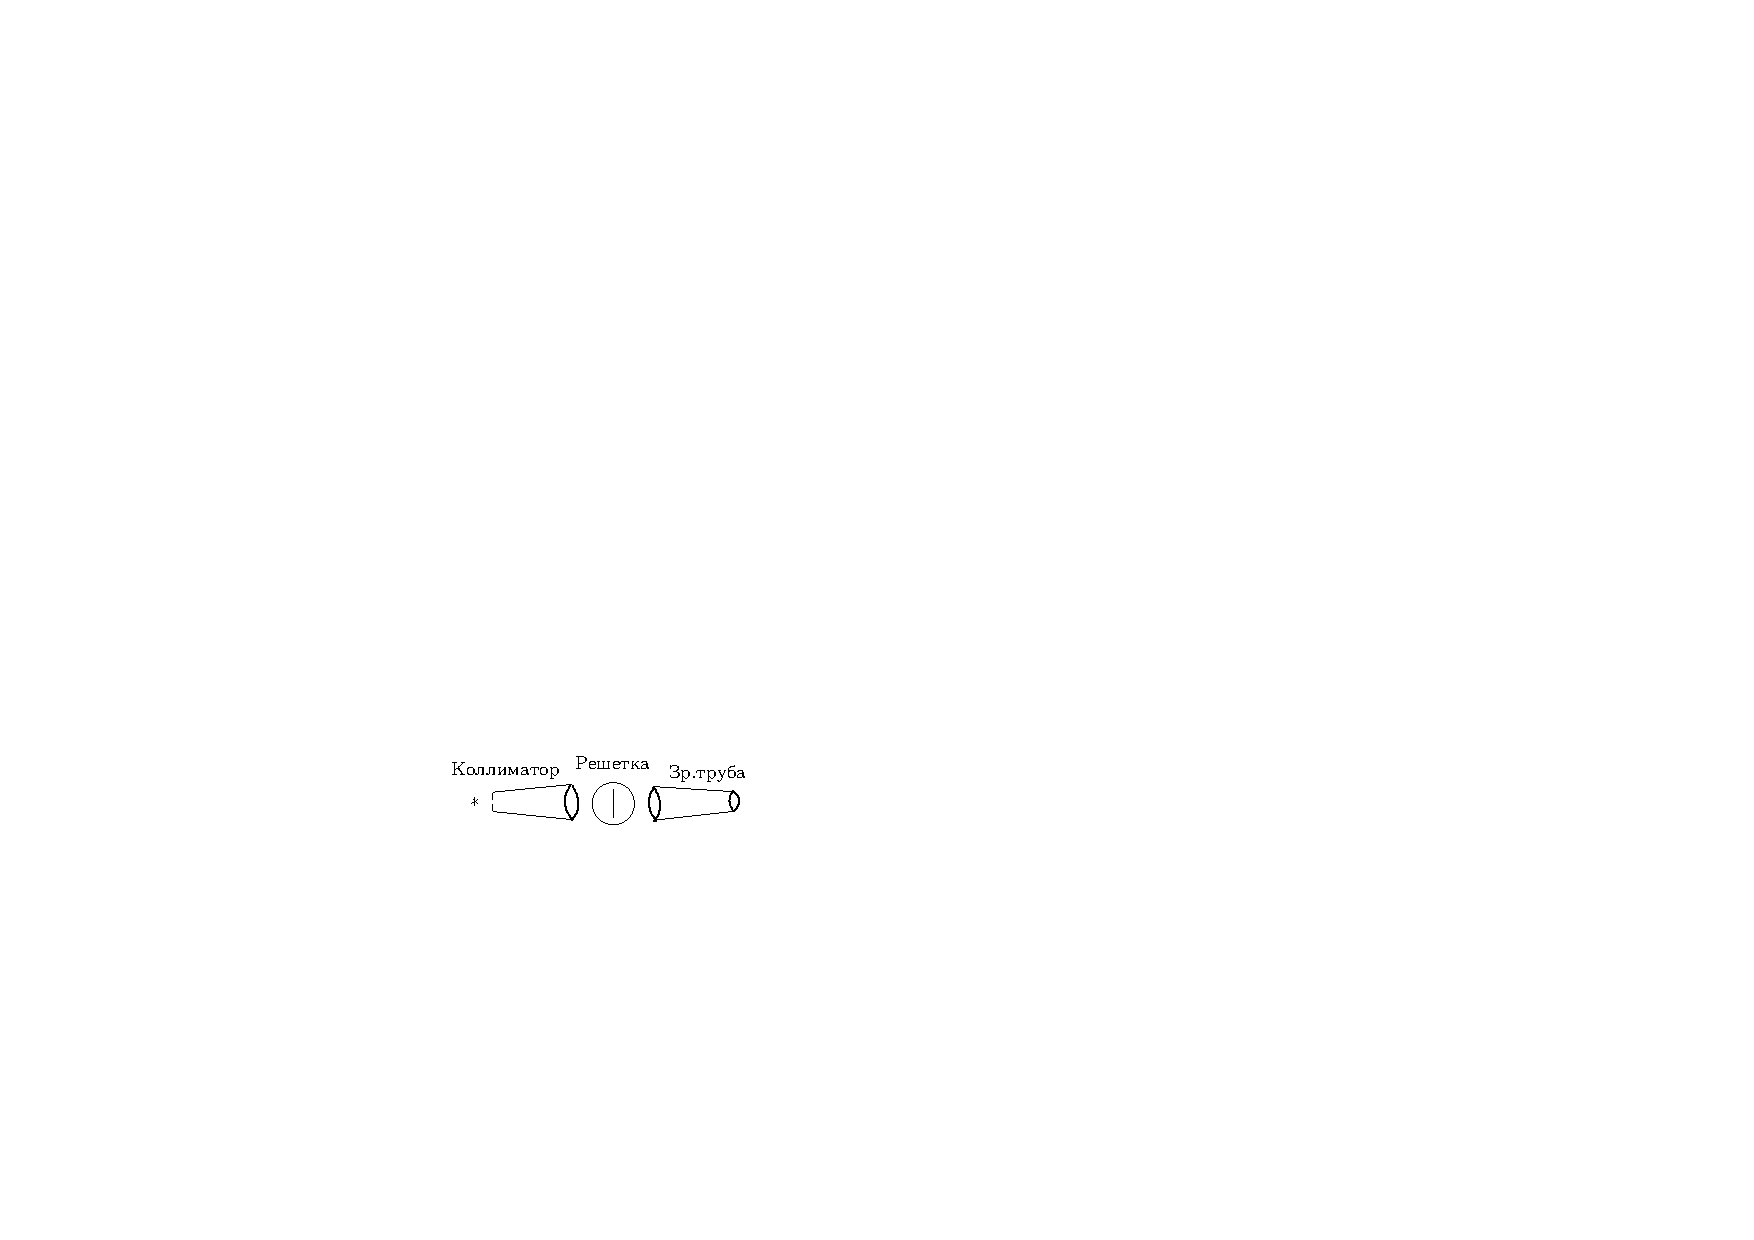
\includegraphics[scale=1.5]{inst.pdf}
	\centering
	\caption{Схема установки.}
	\end{figure}


\newpage
\section{Экспериментальная часть}
\fancyhead[R] {Лабораторная работа №4.4.1}
\fancyhead[L] {Баканова К.В.}
	\subsection{Экспериментальные данные}
		Измерим угловые координаты спектральных линий ртути в $ \pm1 $ порядках, рассчитаем углы дифракции $\varphi_m$. Результаты измерений и вычислений занесем в таблицу 1.

		\begin{table}[h]
			\caption{}
			\begin{tabular}{|p{0.96cm}|p{2.2cm}|p{1.5cm}|p{1.5cm}|p{1.5cm}|p{1.5cm}|p{1.5cm}|p{1.5cm}|p{1.5cm}|}
				\hline
				& фиолетовый & синий  & голубой & зеленый & желтый & желтый & красный & красный \\ \hline
				$ \varphi $& $ 11^{\circ}40' $ & $ 12^{\circ}33' $ & $ 14^{\circ}12' $ & $ 15^{\circ}49' $ & $ 16^{\circ}47' $ & $ 16^{\circ}48' $ & $ 17^{\circ}48' $ & $ 18^{\circ}08' $ \\ \hline
				$\sin \varphi$& 0,2022     & 0,2171 & 0,2451  & 0,2723  & 0,2886 & 0,2888 & 0,3055  & 0,3110  \\ \hline
				$ \lambda $, нм & 404,7      & 435,8  & 491,6   & 546,1   & 577    & 579,1  & 623,4   & 690,7   \\ \hline
			\end{tabular}
						\centering
		\end{table}
					\textbf{       }
					
					
		Для оценки угловой дисперсии решётки определим разности угловых координат линий жёлтого дублета во всех видимых порядках ($ \Delta \lambda = 21  \buildrel _{\circ} \over {\mathrm{A}} $):
		
		\begin{table}[h]
			\caption{}
			\begin{tabular}{|r|c|c|c|}
				\hline
				$m$  & $ \Delta \varphi , ''$  & $D$ exp,  $ 10^{-5} $ рад/$  \buildrel _{\circ} \over {\mathrm{A}}$   & $D$ teor,   $ 10^{-5} $ рад/$  \buildrel _{\circ} \over {\mathrm{A}}$   \\ \hline
				1  &50      & $1,14\pm 0,16$ & $5,22$  \\ \hline
				-1 & 239     &$-5,46\pm0,16$ & $-5,22$ \\ \hline
				2  & 588     &$13,4\pm0,1$ & $12,2$  \\ \hline
				-2 & 548     &$-12,5\pm 0,1$ & $-12,2$ \\ \hline
				3  & 	1350    &$30,9\pm 0,1$ & $29,9$  \\ \hline
				-3 &1332    & $-30,4\pm 0,1$ & $-29,9$ \\ \hline
			\end{tabular}
			\centering
		\end{table}

		Построим график зависимости $\sin \varphi_m$ от длины волны $\lambda$ для $\pm 1$ порядка:
		
			\begin{figure}[h]
	\includegraphics[scale=0.55]{graph1.pdf}
	\centering
	\caption{Зависимость $\lambda$ от $\sin \varphi_m$.}
	\end{figure}
	
		Определим по углу наклона графика период решётки:
		\begin{equation}
			d = (2,1\pm 0,2) \ \text{мкм}.
		\end{equation}
		\textbf{       }
	
		Оценим разрешимый спектральный интервал:
		\begin{equation}
			\delta\lambda \approx \Delta\varphi/D = 2 \buildrel _{\circ} \over {\mathrm{A}};
		\end{equation}
		\textbf{       }
		
		Разрешающая способность будет равна:
		\begin{equation}
			R \approx \frac{\lambda}{\delta\lambda}
		\end{equation}
		\textbf{       }
		
		Число эффективно работающих штрихов решётки:
		\begin{equation}
			N \approx R/m = 288
		\end{equation}
		\textbf{       }
		
		Эффективный размер:
		\begin{equation}
			l \approx Nd = 6\; \text{мм.}
		\end{equation}
		
\section{Выводы}
\fancyhead[R] {Лабораторная работа №4.4.1}
\fancyhead[L] {Баканова К.В.}
	В данной лабораторной работе мы исследовали спектральные линии ртути, вследствие чего смогли определить шаг решётки, её угловую дисперсию и её эффективный размер. Полученные нами результаты оказались близки к теоретическим, за исключением первого порядка.



\end{document}
